\documentclass[
  a5paper,10pt,           % Basic geometry and type size
  dvipsnames              % To be passed to the xcolor package
]{book}
\usepackage{etex}         % Reserve room for 32 additional insertion classes
\reserveinserts{32}       %% that will not be taken away by `\newcount` et al.
\usepackage{polyglossia}  % Hyphenation
\setmainlanguage{english}
\setotherlanguages{french,italian,german}
\usepackage{placeins}     % Float barriers
\usepackage{tikz}         % Diagrams
\usetikzlibrary{trees,arrows}
\usepackage{fancyvrb}     % Manually colored verbatim
\usepackage{float}        % Non-floating figures
\usepackage{url}          % URLs
\usepackage{tabularx}     % Tables
\usepackage{booktabs}
\usepackage{latexsym}     % Additional LaTeX symbols
\usepackage[              % Bibliography
  backend=biber,
  style=numeric,
  citestyle=numeric-comp,
  sorting=none,
  backref=true
]{biblatex}
\addbibresource{main.bib}
\usepackage[nottoc]{tocbibind}
\usepackage{makeidx}      % Index
\makeindex
\usepackage{varwidth}     % Variable-width minipages
\usepackage{./main}       % Markup and design
% Chapter 1
\defacronym[cite=asa63]{ASCII}{the American Standard Code for Information Interchange}
\defacronym{ASA}{the American Standard Association}
\defacronym{IBM}{the International Business Machines Corporation}
\defacronym{FORTRAN}{the FORmula TRANslator}
\defacronym{COBOL}{the COmmon Business-Oriented Language}
\defacronym{ISO}{the International Organization for Standardization}
\defacronym{IEC}{the International Electrotechnical Commission}
\defacronym[cite=iso93]{UCS}{the Universal multiple-octet coded Character Set}
\defacronym{BMP}{the Basic Multilingual Plane}
\defacronym{UTF}{the \acroshort{UCS} Transformation Format}
\defacronym{BOM}{the Byte Order Mask character}
\defacronym{EBCDIC}{the Extended Binary Coded Decimal Interchange Code}
\defacronym{PC}{the \acroshort{IBM} Personal Computer}
\defacronym{JIS}{the Japanese Industrial Standards encoding}
\defacronym{EUC}{the Extended Unix Code}
\defacronym{SR}{Sound Recognition}
\defacronym{OCR}{Optical Character Recognition}
\defacronym{IME}{Input Method Editor}
\defacronym{GUI}{Graphical User Interface}
\defacronym{CLI}{Command Line Interface}
\defacronym[extra={Also known as the Berkeley Unix}]%
  {BSD}{the Berkeley Software Distribution}
\defacronym{joe}{the Joe's Own Editor}
\defacronym{pico}{the PIne COmposer}
\defacronym{emacs}{the Eventually Munches All Computer Storage editor}
\defacronym{vi}{the Visual Interactive editor}
\defacronym{vim}{\acroshort{vi} IMproved}
\defacronym[short-plural={es}]{DPS}{Document Preparation System}
\defacronym[cite={iso08}]{PDF}{the Portable Document Format}
\defacronym[cite={iso12}]{OOXML}{the Office Open XML format}
\defacronym[cite={iso15}]{ODF}{the Open Document Format for office applications}
% Chapter 2
\defacronym{GML}{the General Markup Language}
\defacronym{SGML}{the Standard General Markup Language}
\defacronym{DTD}{Document Type Declaration}
\defacronym[cite=bray98]{XML}{the eXtensible Markup Language}
\defacronym{Relax NG}{the REgular LAnguage for \acronym{XML} New Generation}
\defacronym[cite=duerst05]{IRI}{the Internationalized Resource Identifier}
\defacronym[cite=lie96]{CSS}{the Cascading Style Sheets language}
\defacronym{TEI}{the Text Encoding Initiative}
\defacronym{MathML}{the Mathematical Markup Language}
\defacronym{SVG}{the Scalable Vector Graphics language}
\defacronym[foreign={\foreign[french]{la Conseil Européen pour la Recherche
  Nucléaire}}]{CERN}{the European Organization for Nuclear Research}
\defacronym{HTML}{the HyperText Markup Language}
\defacronym{W3C}{the World Wide Web Consortium}
\defacronym[cite=pemberton00]{XHTML}{the eXtensible Hypertext Markup Language}
\defacronym[cite=lassira99]{RDF}{the Resource Description Framework}
\defacronym{DC}{the Dublin Core}
\defacronym{FOAF}{Friend Or A Foe}
\defacronym[cite=mcguinness04]{OWL}{the Web Ontology Language}
\defacronym{JSON}{the JavaScript Object Notation}
\defacronym{LD}{Linked Data}
\defacronym[cite=sporny14]{JSON-LD}{\acronym{JSON} for \acronym{LD}}
\defacronym[cite=adida08]{RDFa}{\acronym{RDF} in attributes}
\defacronym{WYSIWYG}{What You See Is What You Get}
\defacronym{GNU}{\acroflat{GNU} is Not Unix}
\defacronym{API}{Application Programming Interface}
\defacronym{ECMA}{the European Computer Manufacturers Association}
\mdefacronym{ATnT}{AT\scamp T}{the American Telephone and Telegraph corporation}
\defacronym{DTP}{DeskTop Publishing}
% Bibliography
\defacronym{USA}{the United States of America}
\defacronym{MA}{Massachusetts}
\defacronym{NY}{New York}
\defacronym{TC}{a Technical Committee}
\defacronym{JTC}{a Joint \acronym{TC}}
\defacronym{SC}{a SubCommittee}
\defacronym{WG}{a Working Group}
\defacronym{RFC}{a Request For Comments}
\defacronym{CA}{California}
\defacronym{CLDR}{the Common Locale Data Repository}
        % Acronyms
\begin{document}
\frontmatter
\title{Electronic Document Preparation\\Pocket Primer}
\author{Vít Novotný}
\maketitle
\tableofcontents
\mainmatter
\fakechapter{Foreword}
With the advent of the digital age, typesetting has become available to
virtually anyone equipped with a personal computer. Beautiful text documents can
now be crafted using free and consumer-grade software, which often obviates the
need for the involvement of a professional designer and typesetter. The level
playing field of the Internet coupled with the rising popularity of digital-only
documents then allows the author to bypass the publisher as well, if they so
wish, without jeopardizing their chance of recognition.

This aim of this book is to provide a general overview of the tools and
techniques tied with writing, designing, typesetting, and distributing text
documents---the most universal form of knowledge preservation and transfer
invented by man. Each chapter describes one discrete step of document
preparation along with practical examples and references to literature for those
interested in further study of the subject matter.

Every chapter is filled with examples that illustrate the subject matter. These
should be consulted whenever the concepts described in the text are unclear to
the reader. Although care was taken not to favor any computing environment,
some examples feature Unix utilities, which have no suitable counterpart in
operating systems such as Windows. To try these examples out, the reader is
advised to install a Unix-like environment, such as the Windows Cygwin, on their
local machine or to use a \Unix, such as \Linux.

\chapter{Writing}
The essence of a document is the idea it represents. In the case of a text
document, this idea is articulated through speech, which is transcribed using
text, optionally accompanied by figures, and then laid out on a sheet of paper
according to a design. Since the text is typically independent on the design,
whose task is to support and elicit the internal structure of the text, it is
writing that is the logical first step in the text document creation.

\begin{figure}
  \input examples/01/trichter
  \caption{Exceptions that prove the rule about the separation of text and
    design can sometimes be encountered in poetry. Above is \person{Christian
    Morgenstern}'s \foreign[german]{\work{Trichter}}, where the text and its
    form are intimately intertwined.}
\end{figure}

The essentials of writing in any given natural language include \termpl*{grammar
rule}\index{writing rules!grammar}, which specify the structure of spoken
language, and \termpl*{orthographic rule}\index{writing rules!ortography}, which
impose additional requirements on written text. The complexity of either set of
rules depends entirely on the language in question. Some writing systems, such
as the Japanese kanji, are not phonographic and the correspondence between
the spoken words and the written symbols needs to be memorized by the writer on
a word-to-word basis. Other languages may use vastly different grammar rules for
speaking and for writing, which means that a spoken sentence needs to be
translated first before writing down. A writer needs to recognize these
specifics.

On top of grammar and orthographic rules stand \termpl{style guide}, which, in
order to improve consistency, codify how common language patterns are encoded.
More comprehensive style guides---such as \work{the Chicago Manual of Style} or
\work{the Oxford Style Manual}\footnote{
  This document was prepared in accordance with \person{William Strunk}'s
  \work{Elements of Style}, an American English style guide for general use. 
}---often go beyond writing and provide guidelines on design and typesetting as
well, making them an indispensable reference on the editorial tradition.

Above all stand the \termpl*{typographic rule}\index{writing rules!typography},
which specify how the resulting document should be typeset so that it doesn't
disturb the eye of the reader. These, as well as the orthographic rules on
hyphenation, can be left out of consideration during writing, as it is the page
that should be formed around the writing and not the other way around.

\section{Text Processing}
Originally the domain of the pen, the quill, the stylus, and the more recent
typewriter machine, manuscripts of today are produced chiefly using the personal
computer and stored in \termpl{text file}. The discipline of creating and
manipulating digital text is called \term{text processing} and will be the focus
of this section.

\subsection{Character Encoding}
Although computing at its most primal has no use for anything but numbers, it
has nevertheless been accompanied by text from the very outset. Even the
earliest computers from 1950s were programmed with both raw machine code and
the text programming languages of \acronym{FORTRAN} and \acronym{COBOL}. The
digital representation of letters, digits and other characters was initially
closely tied to each specific application and processor architecture, but with
the advent of networking in 1960s, mutual intelligibility became a point of
concern.\iffalse\footnote{
  \Acronym{EBCDIC} by \acronym{IBM} was the default encoding on
  \acroshort{IBM}'s System/360 mainframes and was in active use until the
  introduction of \acronym{PC} in 1981. In countries using Chinese ideographs,
  special encodings, such as Big5, \acronym{JIS}, and \acronym{EUC}, are used to
  this day. For brevity, the text focuses on the main stream of international
  encodings.}\fi
\ ``We had over sixty different ways to represent characters in
computers. It was a real Tower of Babel,'' explains \cite{brandel99}
\person{Bob Berner}, an American computer scientist who worked at \acronym{IBM}
during 1956--1962 and who drafted \acronym{ASCII}---a
\term{character encoding} from \citeyear{asa63} that unified the industry and
enabled computer networking on large scale.

\subsubsection{ASCII}
In \acronym{ASCII}, every character is represented by a number from zero to 127,
which is transformed to a seven-bit integer called a \term{character code}.
These 128 codes are used to encode \termpl{printable character}---spanning the
letters of the English alphabet, digits, punctuation, and other symbols---and
\termpl{control code}, as depicted in Table \ref{tab:ascii}.  Unlike printable
characters, control codes have no fixed visual representation and they were used
to implement application-specific communication protocols and text formatting;
their precise semantics were defined in the much later standard of
\acroshort{ISO}~646 from \citeyear{iso72} \cite{iso72}. Unconstrained by the
bandwidth and the storage limitations of the 1960s and 1970s, today's
communication protocols and text formats gravitate towards markup constructed
from printable characters, which, unlike control codes, are easy to read and
write by humans.

\begin{table}
  \input examples/01/ascii
  \caption{The \acronym{ASCII} encoding, as specified in the \citeyear{asa86}
    revision of the standard \cite{asa86}.}
  \label{tab:ascii}
\end{table}

\begin{table}
  \input examples/01/utf8
  \caption{The \acroshort{UTF}-8 encoding. Each \textvisiblespace\ represents
    one bit of the \acroshort{UCS} code point in binary.}
  \label{tab:utf8}
\end{table}

\begin{table}
  \input examples/01/utf8-example
  \caption{An example of the \acroshort{UTF}-8 encoding}
  \label{tab:utf8-example}
\end{table}

%%% ASCII, Other Standards
%%%   <https://en.wikipedia.org/wiki/ASCII#Other_standards>
%%%   <https://en.wikipedia.org/wiki/ISO/IEC_8859-2#External_links>
%%%
%%% Character histories: notes on some Ascii code positions
%%%   <http://www.cs.tut.fi/~jkorpela/latin1/ascii-hist.html>
%%%
%%% ASCII: American Standard Code for Information Infiltration
%%%   <http://worldpowersystems.com/J/codes/>
%%%
%%% Encyclopedia of Computer Science, 4th edition
%%%   <https://dl.acm.org/ralston.cfm?CFID=698031209&CFTOKEN=46500462>
%%%
%%% Theoretical Foundation of Regular Expressions and Text Editors
%%%   <http://citeseerx.ist.psu.edu/viewdoc/download?rep=rep1&type=pdf&doi=10.1.1.126.9920>
%%%
%%% A History of Scientific Text Processing at CERN
%%%   <http://ref.web.cern.ch/ref/CERN/CNL/2001/001/tp_history/>
%%%
%%% When and how did text enter the world of computing, eventually to be
%%% standardized as ASCII in 1963? <http://qr.ae/RHFEzE>
%%%
%%% IBM's Early Computers: A Technical History
%%%   <http://www.amazon.com/IBMs-Early-Computers-Technical-Computing/dp/0262523930>

The following properties make it easy to manipulate and reason about character
strings encoded in \acronym{ASCII}:
\begin{itemize}
  \item Each character is represented by exactly seven bits. This makes it easy
    to allocate space for character strings of fixed length, to measure the
    number of characters stored in a memory region, and to perform basic
    operations, such as adjacent character retrieval or text truncation.
  \item Characters are alphabetically ordered. Character strings can therefore
    be collated by comparing character code binary values.
  \item Lowercase and uppercase letters, digits and control codes form
    contiguous ranges of character codes, simplifying classification.
  \item There is precisely one way to encode any printable character. The
    conversion between the lower- and uppercase letters is a matter of
    inverting one bit.
\end{itemize}
This comes at the expense of support for non-English writing systems. As a
temporary workaround, a set of \acroshort{ASCII} derivatives that replaced the
less-needed characters of \# \$ @ [ \textbackslash\ ] \textasciicircum\ ` \{ |
\} and \textasciitilde\ for international characters was specified in the
\acroshort{ISO}~646 standard \cite{iso72} from \citeyear{iso72}.

\subsubsection{Eight-bit Encodings}
With the byte size stabilizing at eight bits, new character encodings emerged
that were based on \acronym{ASCII} and utilized the additional bit to encode
characters of non-English writing systems while retaining complete backwards
compatibility with \acroshort{ASCII}. Beside the numerous vendor-specific
encodings (called \termpl{code page}), a set of 15 eight-bit encodings covering
all major modern writing systems whose characters fit within the space of 128
additional combinations was standardized in the
\acroshort{ISO}/\acroshort{IEC}~8859 series released during 1986--2001.

  % Show a time diagram of Czech encodings
  %   <http://luki.sdf-eu.org/txt/cs-encodings-faq.html>

Compared to \acronym{ASCII}, eight-bit encodings introduced an additional level
of complexity to text processing:
\begin{itemize}
  \item Each character is exactly eight bits wide. The manipulation with strings
    is therefore as straightforward as with \acronym{ASCII}.
  \item Character strings can no longer be collated by character code
    comparison. Each encoding requires a separate mapping from character codes
    to sorting weights.
  \item Classes of characters, such as uppercase and lowercase letters or
    punctuation, no longer form contiguous ranges and their position varies
    among encodings. This impedes character classification.
  \item Idiosyncrasies, such as the ligature of æ and invisible hyphenation
    hints, are included in several encodings, which makes it more difficult to
    determine character string equivalence. Among encodings that contain lower-
    and uppercase letters, the algorithms for case conversion vary.
  \item There exists no standard mechanism to detect which encoding is being
    used. The distinction needs to be done on the application level using either
    heuristics or additional metadata. Consequently, no standard mechanism
    exists to use different character encodings within a single text document.
\end{itemize}
A portion of this complexity is inherent in the task of encoding the characters
of all modern writing systems, but the overhead caused by the character encoding
fragmentation proved to be hurtful and unnecessary.

\subsubsection{The Universal Character Set and Unicode}
The continual increase in the available bandwidth and storage led to the
creation of the standards of Unicode \cite{unicode91,unicode92} and
\acronym{UCS} in an attempt to create a text encoding that would
contain the characters of all the world's living languages and succeed
\acronym{ASCII} as the \foreign[italian]{lingua franca} of text interchange.

\Acronym{UCS} is an ever-expanding catalogue of characters from writing systems
both modern and ancient, and symbols ranging from diacritical marks,
punctuation, and ideograms to mahjong tiles, alchemical symbols, and the ancient
Greek musical notation. Each of these characters is assigned a number, called
a \term{code point}, ranging from 0 to 2,147,483,647 (\hexa{7FFFFFFF}) with the
numbers of the most common characters in the range from 0 to 65,535
(\hexa{FFFF}) called \acronym{BMP}. The smallest unit of division in
\acronym{UCS} are \termpl*{block}\acroindex[!block]{UCS}, which contain 256
thematically related characters. \Acronym{UCS} encodings map character numbers
to binary character codes.

Three major encodings\footnote{
  Notable are also the seven-bit encodings of \acroshort{UTF}-7
  \acroindex[!UTF-7@\acroshort{UTF}-7]{UTF} and \inx{Punycode}, which bring
  Unicode support to protocols that were designed with the seven-bit
  \acroshort{ASCII} in mind, such as e-mail.}
are specified in the \acronym{UCS} standard and its amendments
\cite{iso93:am1,iso93:am2}:
\begin{description}
  \item[\acroshort{UTF}-32]\acroindex[!UTF-32@{\acroshort{UTF}-32}]{UTF}Directly
    encodes \acronym{UCS} characters by transforming their code points to
    four-byte integers. \acroshort{UTF}-32 is also known as
    \acroshort{UCS}-4\acroindex[!UCS-4@{\acroshort{UCS}-4}]{UCS}.
  \item[\acroshort{UTF}-16]\acroindex[!UTF-16@{\acroshort{UTF}-16}]{UTF}
    Directly encodes characters within \acronym{BMP} by transforming their code
    points to two-byte integers. Code points in the range from 65,536 to
    1,114,111 (\mbox{\hexa{010000}--\hexa{10FFFF}}) are transformed into a pair
    of two-byte integers, called a \term{surrogate pair}, ranging from
    55,296 to 57,343 (\mbox{\hexa{DC00}--\hexa{DFFF}}). To enable the
    \acroshort{UTF}-16 encoding, the code points in the surrogate pair range
    will never be assigned. The same applies to code points greater than
    1,114,111 (\hexa{10FFFF}), which allows \acroshort{UTF}-16 to encode any
    \acroshort{UCS} character.
  \item[\acroshort{UTF}-8]\acroindex[!UTF-8@{\acroshort{UTF}-8}]{UTF}
    Directly transforms code points ranging from 0 to 127 (\hexa{7F}) to one-byte
    integers. Since the first \acroshort{UCS} block of the \acroshort{BMP}
    matches \acronym{ASCII}, any text encoded in eight-bit \acroshort{ASCII} is
    therefore also encoded in \acroshort{UTF}-8. Code points in the range from
    127 to 1,114,111 (\mbox{\hexa{00007F}--\hexa{10FFFF}}) are transformed into
    two to four one-byte integers ranging from 128 to 253
    (\mbox{\hexa{80}--\hexa{FD}}). The encoding is illustrated in tables
    \ref{tab:utf8} and \ref{tab:utf8-example}.
\end{description}
\acroshort{UTF}-32 is primarily used for the internal representation of
individual \acronym{UCS} characters inside programs, \acroshort{UTF}-16 fulfills
a similar role in applications that only work with \acronym{BMP}, and
\acroshort{UTF}-8 is used for text storage and interchange. Since 2010, the
majority of text content on the Web is encoded in \acroshort{ASCII} and
\acroshort{UTF}-8 \cite{qsuccess15}.

Originally a competing standard, Unicode underwent a merger with \acronym{UCS}
in version 1.1 and since then, the standards have been kept closely
synchronised. Unicode is a superset of \acronym{UCS}, which defines additional
information about \acronym{UCS} characters---such as their general category,
directionality, case, or numeric value \cite[sec.\,3.5,~ch.\,4]{unicode15}---,
various text processing algorithms, and implementation guidelines.

\begin{figure}
  \ffootnote{One of the design goals of \acroshort{UCS} was to avoid assigning
    code points to different glyphs that carry the same meaning. As a result,
    the visually distinctive Han characters used in the East Asian countries
    of China, Japan, Korea, and Vietnam were merged into a set of 75,960
    ideograms in a process referred to as the \term{Han Unification}. This
    simplifies text processing, but also makes it impossible to encode a text
    in multiple East Asian languages without having to rely on external markup
    to select appropriate regional fonts. As a result, a derivative of
    \acronym{UCS} that doesn't implement the Han Unification was developed for
    use in operating systems based on \acronym{TRON} and is used in the East
    Asia alongside \acronym{UCS} and region-specific encodings.}
  \input examples/01/unihan
  \caption{Several Han characters in the traditional Chinese, Japanese,
    Korean, and Vietnamese variants}
\end{figure}

With regards to text processing, Unicode and \acronym{UCS} represent a
compromise between the simplicity of the seven-bit \acronym{ASCII} and the
heterogeneity of eight-bit encodings:
\begin{itemize}
  \item If simple text manipulation is preferred over space efficiency, each
    character can be made exactly two or four bytes wide using the
    \acroshort{UTF}-16 and \acroshort{UTF}-32 encodings.
  \item Although character strings can not be collated by a simple character
    code comparison, a collation algorithm is defined in the Unicode
    specification \cite{unicode15:collation} and collation tables for major
    locales \cite{unicode15:cldr} are maintained by the Unicode Consortium.
  \item Classes of characters---such as uppercase letters, lowercase letters,
    numbers, and punctuation---do not form contiguous ranges, but their position
    is directly specified by the standard \cite[sec.\,4.5]{unicode15}.
  \item Although idiosyncrasies---such as ligatures, invisible hyphenation
    hints, and combining characters---are present in \acronym{UCS}, explicit
    normalization algorithms for character string equivalence testing are
    specified by the standard \cite[sec.\,2.12]{unicode15}. An algorithm
    for case conversion is also specified \cite[sec.\,3.13]{unicode15}.
    \index{Unicode!normalization}\index{Unicode!case conversion}
  \item The \ucs[FEFF]{Byte Order Mark} character can be inserted at the
    beginning of a text as a signature of Unicode encodings. As the name
    suggests, the order in which the \hexa{FE} and \hexa{FF} bytes arrive also
    indicates the order of bytes (called \term{endianity}) that was used to
    encode integers. In \acroshort{UTF}-32 and \acroshort{UTF}-16, endianity
    can be chosen arbitrarily by the encoding application. In \acroshort{UTF}-8,
    one-byte integers are used and the notion of endianity is therefore
    meaningless.
\end{itemize}

\begin{figure}
  \input examples/01/combining-chars
  \caption{Some \acroshort{UCS} characters can be either input as a single
    entity or composed from several combining characters. With regards to the
    Unicode normalization forms, all of the above representations are
    canonically equivalent.}
\end{figure}

\begin{figure}
  \centerline{\code[sh]{iconv -f latin2 -t utf8 -- old.txt > new.txt}}
  \caption{Text files can be converted between encodings using the
    \cliutil{iconv} command-line tool. The sample code shows the file
    \filename{old.txt} being converted from the
    \acroshort{ISO}/\acroshort{IEC}~8859-2 encoding to \mbox{\acroshort{UTF}-8}.
    The result of the conversion is stored in the file \filename{new.txt}.}
\end{figure}

%%% Setting collation order in shell sort
%%%   <http://superuser.com/a/414408/136765>
%%%
%%% Unicode 101: An Introduction to the Unicode Standard
%%%   <http://www.interproinc.com/blog/unicode-101-introduction-unicode-standard>
%%%
%%% Unicode Implementation levels
%%%   <http://www.cl.cam.ac.uk/~mgk25/unicode.html#levels>
%%%
%%% Unification of the Unicode Standard and ISO 10646
%%%   <http://www.unicode.org/versions/Unicode1.0.0/V2ch01.pdf>
%%%
%%% Unicode 88 <http://unicode.org/history/unicode88.pdf>
%%% Unicode equivalence <https://en.wikipedia.org/wiki/Unicode_equivalence>
%%%
%%% Plane (Unicode):
%%%   <https://en.wikipedia.org/wiki/Plane_(Unicode)#Basic_Multilingual_Plane>

\subsection{Text Input}
To insert text into a document, it is necessary to use an input device. In case
of personal computers, this is typically a computer keyboard and a mouse,
although the ongoing research in the areas of \acronym{SR} and \acronym{OCR}
makes it possible to use a microphone or a tablet as well. On hand-held devices,
the use of either a numeric keypad or a touch-screen is more typical.

An operating system will typically provide one or more input methods for each
input device through a component commonly referred to as the \acronym{IME}. The
\acroshort{ASCII} encoding was developed with typewriters and teleprinters in
mind and, as their direct descendant, the standard computer keyboard provides
support for all \acroshort{ASCII} characters. This doesn't apply to the much
larger \acronym{UCS} and it is the task of an \acronym{IME} to provide a
mechanism for the creation and selection of keyboard layouts that will allow the
user to input any \acronym{UCS} character. Some programs may provide input
methods of their own.

\begin{figure}
  \centerline{\includegraphics[width=0.75\textwidth]%
    {examples/01/google-pinyin.png}}
  \caption{Text input methods are not limited to keyboard layouts. Software that
    allows for the input of non-Latin characters on a keyboard through reversed
    romanization can often be the best option for writing systems with a large
    number of characters. Above is the \inx{Google Pinyin} input method for the
    Android operating system, which makes it possible to input Chinese
    characters using the \inx{pinyin} phonetic system.}
  % TODO: Získat lepší screenshot
\end{figure}

\begin{figure}
  \input examples/01/composeKey
  \caption{The \key{Compose}\index{Compose@\displaykey{Compose}} key followed by
    a mnemonic sequence of \acroshort{ASCII} characters produces a
    \acroshort{UCS} character. Although originally a physical key, \key{Compose}
    is not available on modern \acroshort{PC} and Apple keyboards and is usually
    mapped to a less-used key, such as the right \key{Ctrl} or \key{Super} key.
    \key{Compose} is natively supported on \Unices\ using the \inx{X Window
    System}. On other operating systems, support can be added by installing
    third-party software.}
\end{figure}

\begin{figure}
  \input examples/01/altCodes
  \caption{On the Windows operating system, holding the \key{Alt} key and typing
    a sequence of numbers produces a character with the corresponding number
    from either an \acroshort{IBM} code page, if the number has no leading zero,
    or from a Windows code page otherwise. The code pages vary depending on the
    current locale; in English locales, the \acroshort{IBM} code page~437
    and the Windows code page~1252 are used. After a Windows Registry
    modification, it is also possible to directly produce \acroshort{UCS}
    characters by holding the \key{Alt} key and typing the corresponding
    \acroshort{UCS} code point in hexadecimal.}
\end{figure}

\subsection{Text Editors}
A \term{text editor} is an applications, which can be used to create and modify
text files. Entry-level text editors are often distributed with an operating
system and offer little beyond the ability to load, modify and save text files.
Entry-level text editors with a \acronym{GUI} include the \inx{Windows Notepad},
the iOS \inx{TextEdit} in plain text mode, and \inx{Leafpad} for \Linux\ and
\acronym{BSD}. Entry-level text editors with a \acronym{CLI} include
\cliutil{joe}, \acroshort{GNU} \cliutil*{nano}\acroindex[!nano]{GNU}, and
\cliutil{pico}.

More advanced text editors come with the support for \termpl{regular expression}
and \term{version control}---which will be covered in sections \ref{sec:regexs}
and \ref{sec:vcs}---, as well as user modules that extend the base
functionality.  Advanced \acronym{GUI} text editors include \inx{Sublime Text},
\inx{Atom}, and \inx{PSPad}. Advanced \acronym{CLI} text editors include
\cliutil{emacs}, \cliutil{vi}, and \cliutil{vim}. The presented \acronym{CLI}
text editors are especially notorious for their learning curve, whose steepness
is only matched by the power these editors grant to those who wield them.

\subsection{Interactive Document Preparation Systems}
Interactive \acropl{DPS}\acroindex[!interactive]{DPS} are a breed of text
editors that produces fully-formatted text documents instead of (or along with)
text files. The reader is advices to avoid interactive \acropl{DPS} that use
proprietary, undocumented, and obscure file formats which lock the user into
using the respective \acronym{DPS} to open the files reliably. Well-defined
interactive \acronym{DPS} file formats include \acronym{PDF}, \acronym{OOXML},
and \acronym{ODF}.

The primary difference between text editors and \acropl{DPS} is the fact that
the user is expected to use the \acronym{DPS} to mark up, design, and typeset the
resulting text document, whereas with plain text files a multitude of choices is
available at each step of the document preparation process. The self-sufficient
nature of \acropl{DPS} may be a time-saving feature for simpler documents, but
in the case of more complex documents, the markup and typesetting capabilities
of a \acronym{DPS} may not be up to par with those of a dedicated tool.
Interactive \acropl{DPS} include \inx{Apache OpenOffice}, \inx{TextEdit},
\inx{Microsoft Word}, \inx{Scribus}, and \inx{Adobe InDesign}.

\subsection{Regular Expressions}\label{sec:regexs}
The \term{Chomsky hierarchy} is a classification of text production rules
(called \termpl{formal grammar}), which was proposed \cite{chomsky56} in
\citeyear{chomsky56} by the American linguist \person{Noam Chomsky} in his
endeavor to discover a good formal model for the description of natural
languages. The class of \termpl{regular grammar}, which is the least powerful
of the proposed classes, has properties that make it possible to determine the
grammaticality of a text in constant time and space. \Termpl{regular
expression} are a more intuitive reformulation of regular grammars that a writer
can use to find and replace character strings within text.

Since regular expressions are just a formal model, a software implementation
needs to settle on a concrete syntax. One of the earliest standard syntaxes are
\acronym{BRE} and \acronym{ERE} \cite[part~1,~ch.\,9]{iso93:posix2}, which are
supported by most utilities using regular expressions on \Unices. Both syntaxes
are described in Table \ref{tab:regexs}. More extensive syntaxes include the
\acroshort{GNU} extensions of \acronym{BRE} and \acronym{ERE}, the regex syntag
of the \inx{Perl} programming language, and their dialects and derivatives. For
most of these extended syntaxes, the term \term*{regular} is a misnomer, as the
expressions can be used to build grammars that, according to the Chomsky
hierarchy, aren't regular.\footnote{
  A curious reader with a background in formal language theory should direct
  their attention to Perl self-referencing groups and look-aheads, which make it
  a simple matter to create expressions that match non-context-free formal
  languages.
% It is easy to show that the Perl 5 regex of \code{(?=(a(?-1)?b)c)
% a+(b(?-1)?c)} generates the context-sensitive language of $a^nb^nc^n$ for
% arbitrary characters $a,b,c$ with superscripts denoting repetition.
} To disambiguate the term, these expressions are often called
\termpl*[regexes]{regex}\index{regex|see{regular expression}}.

\begin{table}
  \input examples/01/regexs
  \label{tab:regexs}
\end{table}

%%% POSIX.2-1997: Regular Expressions
%%%   <http://pubs.opengroup.org/onlinepubs/007908799/xbd/re.html>

Many regex syntaxes and the software that implements them were designed for the
processing of \acronym{ASCII} text and may behave in surprising ways, when
confronted with \acronym{UCS} characters. The software may assume that each
character is exactly one byte long and fail to recognize any characters that are
longer as a single character, or it may assume that all \acronym{UCS} characters
fall within \acronym{BMP} and exhibit the same problem with characters outside
\acronym{BMP}. More subtle, but no less precarious, can be the lack of support
for Unicode case conversion and normalization algorithms, which makes it
difficult to perform case-insensitive matching and the matching of characters
that can be encoded in several different ways. The lack of awareness of the
invisible characters that can appear in \acronym{UCS} text---such as the
\ucs[200B]{zero width space}, \ucs[200C]{zero width non-joiner}, \ucs[200D]{zero
width joiner}, and \ucs[FEFF]{zero width no-break space}---, is also problematic
and can lead to false negative matches. Conversely, modern regex syntaxes that
implement the Unicode standard for Regular Expressions \cite{unicode13}---such
as those of Perl 5.2 or Java 7---are actively aware of \acronym{UCS} and provide
features that enable the matching of characters based on their general category,
numeric value, directionality, and other properties defined by Unicode, as shown
in Table \ref{tab:unicode-regexs}.

\begin{figure}
  \input examples/01/unicode-regexs
  \caption{An overview of the elements of the Unicode regex syntax as
    implemented by Perl 5.2 and Java 7. The list of Unicode character properties
    is only demonstrative.}
  \label{tab:unicode-regexs}
\end{figure}

The most elementary text processing \acroshort{CLI} tool is \cliutil{grep}%
\footnote{
  The authoritative resource on \cliutil{grep}, \cliutil{sed}, and \cliutil{awk}
  is \citework{dougherty97}, which explains each tool as well as the
  \acroshort{BRE} and \acroshort{ERE} syntaxes in full detail.
}, which makes it possible to search text files for fixed strings and regexes in
default of an advanced text editor. Unless configured otherwise, the tool will
present lines that contain one or more matches to the user. A more advanced
text-processing \acroshort{CLI} tool is \cliutil{sed}, which features a simple
programming language that can be used to arbitrarily transform text files.
\Cliutil{awk} is a \acroshort{CLI} tool that also features a text-processing
programming language, albeit a more advanced one than that of \cliutil{sed}.
Originally developed for the Research Unix during 1973--1977, \cliutil{grep},
\cliutil{sed}, and \cliutil{awk} are available in various flavors for most
operating systems.

%%% The true power of regular expressions
%%%   <https://nikic.github.io/2012/06/15/The-true-power-of-regular-expressions.html>
%%%
%%% Regular Expression Matching Can Be Simple And Fast
%%%   <https://swtch.com/~rsc/regexp/regexp1.html>
%%%
%%% JavaScript has a Unicode problem
%%%   <https://mathiasbynens.be/notes/javascript-unicode>

\section{Version Control}\label{sec:vcs}
When writing a text document, it is ofter useful to have a backup of the
previous versions of files, so that undesirable changes can be reverted whenever
necessary. If more than one person contributes to the document, the ability to
associate these changes with their authors also becomes useful. If beside
writing we consider the markup, the design, and the typesetting of documents, we
will find that some of these tasks can closely resemble programming, which makes
the ability to move between previous versions of our code instrumental to
tracking down programming errors. To aid with this is the goal of \acronym{VCS}.
At its most rudimentary, \acronym{VCS} records changes along with an information
about their author and a short description. These changes can then be browsed,
viewed, and reverted. With a single contributor, \acronym{VCS} are a convenient
alternative to manual archival of individual versions of the document. With
several contributors, \acronym{VCS} become an irreplaceable instrument.

\Acronym{VCS} can be dichotomized based on its architecture, which is either
\term*{centralized}\acroindex[!centralized]{VCS} or \term*{decentralized
\acronym{VCS}}\acroindex[!decentralized]{VCS}. Centralized \acronym{VCS} stores
all versions in a repository located on a remote server. Users then send and
download new versions to and from the server using a client software. The client
software is \term*{thin} in the sense that it does not store more than one
version locally and its operation is fully dependent on the availability of the
server. An example of centralized \acronym{VCS} is \acronym{SVN}\footnote{
  The authoritative resource on \acronym{SVN} is \citework{sussman02},
  affectionately known as \work{the Subversion book}.
}. By comparison, there is no designated server in decentralized \acronym{VCS}
and the users can send and download new versions to and from any other user. The
client software is \term*{thick} in the sense that each user has a local
repository with all the existing versions, which he browse and expand regardless
of the availability of others. The disadvantages of decentralization include the
more complex workflow and the increased opportunity for the users not to share
their new local versions frequently enough, leading to an increased chance of
colliding changes.  Examples of decentralized \acronym{VCS} include \inx{Git},
\inx{Mercurial}, or \inx{Bazaar}.

\begin{figure}
  \input examples/01/svn
\end{figure}

\begin{figure}
  \ffootnote{%
    The reader should note that although it is typical to use a central
    repository, the decentralized architecture of Git makes it possible for
    clients to exchange the contents of their repositories directly.
    Multiple layers of repositories that automatically exchange the latest
    updates can also be created for backup and other purposes.}
  \vspace*{-1mm} % Forcibly align the two diagrams.
  \input examples/01/git
  \vspace*{4in}  %% Remove if the float positions change.
\end{figure}

Although \acronym{VCS} can be used to keep track of any kind of files, they are
typically geared towards text files, which can be easily displayed along with
the list of changes between two versions. However, most interactive \acropl{DPS}
do not produce text files and the use of traditional \acronym{VCS} would
negatively impact the user experience. As a counter-measure, some \acropl{DPS}
include \acronym{VCS} of their own, which can take the form of an internal
function that records the changes directly into the output file, a separate
\acronym{VCS} that provides a special support for the file format used by the
\acronym{DPS}---such as \inx{Tortoise \acroshort{SVN}} does for Microsoft Office
documents---, or a web service that enables real-time interactive
collaboration---such as \inx{Office Online} or \inx{Google Docs}.

  % Tortoise SVN diffing Microsoft Office documents
  % Revision control in Apache OpenOffice and Microsoft Word

%%% Git porcelains <http://stackoverflow.com/a/6978402>
%%% Pushing an existing Git repository to SVN
%%%   <http://stackoverflow.com/a/772881/657401>

\chapter{Markup}
A manuscript can consist of a seamless river of words and still make perfect
sense to the author. To truly capture its meaning in a clear and unambiguous
manner, however, the manuscript will often need to be supplemented with a set of
annotations. At a more basic level, this refers to the compliance with the
orthographic rules---such as the correct spelling, capitalization, word breaks,
and punctuation---that are specific to the language of the document.  It is not
at all unreasonable to expect that this basic compliance should be already met
by the manuscript. At a higher level, this consists of discovering and marking
up the inner order and logic of the text, so that the resulting document can
later be typeset in a way that visually reflects its structure.

More often than not, the writing and marking up of a text are two inseparably
connected activities performed in parallel rather than in succession.
Nevertheless, each represents a distinct concept: Writing is the process of
breaking ideas into fragmented strings of words, which the markup reassembles
back into meaningful units of linguistic thought waiting to be brought to life
by a designer.

\index{markup!logical|(}\index{markup!presentation|(}
Markup can be created using a variety of \termpl*{markup language}. Aside from
\term*{logical markup}, which captures the logical structure of a document,
markup languages may also provide \term*{presentation markup}, which directly
impacts the visual properties of the document but carries no semantic
information. The usage of presentation markup makes it impossible to separate
the markup from the design and to capture the logic of the text. As a result,
the consistency in the design of each logical part of the document needs to be
ensured manually, and future changes of design become error-prone and tedious.
In this regard, logical markup is to design what style guides are to writing: a
means of ensuring consistency that should be used whenever possible.
\index{markup!logical|)}\index{markup!presentation|)}

\section{Meta Markup Languages}
\subsection{The General Markup Language}
The situation engulfing digital typesetting was growing increasingly frustrating
for publishers in the 1960s. The markup languages used by different typesetting
systems varied wildly, and once a publisher had a large collection of documents
typeset via a given company, switching to another one could be very costly
venture. The companies would take advantage of this situation, causing their
prices to skyrocket. As a result of that, a demand for a universal markup
language emerged.

This demand was met by a project developed\footnote{
  More information about the project can be found within
  \citework{goldfarb96} and \citework[SGML: The Reason Why and the First
  Published Hint]{goldfarb97:whySGML}.
} at the Cambridge Scientific Center of \acronym{IBM} in the early 1970s. The
project aimed at imbuing a text editor with the ability to query, edit, and
display documents from a repository to allow the usage of computers in legal
practice. Very early on in the development process, it became clear that the
crux was going to be the markup languages in which the documents were written.
These languages were not unified and many of them comprised largely presentation
markup, which made information retrieval impossible without the use of
heuristics. To resolve these issues, a unifying markup language called
\acronym{GML} was drafted. The language was released \cite{goldfarb81}
to the public in \citeyear{goldfarb81} and finally standardized in
\citeyear{iso86} as \acronym{SGML}\footnote{
  The authoritative resource on \acronym{SGML} is \citework{goldfarb91}, which
  includes the full text of the standard bearing extensive annotations.
} \cite{iso86}.

\Acronym{SGML} documents consist of text mixed with \termpl*{tag}%
\acroindex[!tag]{SGML}, which delimit meaningful sections of the document called
\termpl*{element}\acroindex[!element]{SGML}. Elements can carry additional
information in \termpl*{attribute}\acroindex[!attribute]{SGML}. Additionally,
\acronym{SGML} documents may contain miscellaneous instructions for the program
that is processing it, as well as human-readable comments. Repeated strings of
text can be declared as \termpl*[entities]{entity} \acroindex[!entity]{SGML}
that can consequently be used throughout the document in place of the original
strings.

Although the described structure is shared by all \acronym{SGML} documents, the
actual syntax, as well as the restrictions with regards to the contents and the
attributes of individual elements, are declared within a \acronym{DTD}, which
can be different for each document. It is worth noting that a \acronym{DTD} only
declares the syntax of an \acroshort{SGML} document; the semantics of the
individual elements and their attributes are left to the interpretation of the
program processing the document. The syntax and the constraints imposed by a
\acronym{DTD} define an \term*{application of \acronym{SGML}}
\acroindex[!application]{SGML}. An \acronym{SGML} document is considered to be a
valid instance of an \acroshort{SGML} application, when it conforms to the
respective \acronym{DTD}.

\subsection{The Extensible Markup Language}
Although \acronym{SGML} was designed to be the general format for data exchange,
the complexity of the specification and the lack of support for Unicode proved
to be a major hindrance preventing its wider adoption and tool development. As a
response, \acronym{W3C} published a specification of \acronym{XML} in
\citeyear{bray98}. Along with the introduction of \acronym{XML}, the
\acroshort{SGML} specification received a technical corrigendum
\cite{goldfarb97:webSGML}, which turned \acronym{XML} into a proper subset of
\acronym{SGML} restrained by an \acroshort{SGML} \acronym{DTD}.

\begin{figure}
  \inputcode[xml]{examples/02/recipe.xml}
  \caption{An example \acronym{XML} document\filenamecap{recipe.xml}}
  \label{fig:recipe}\bigskip
  \inputcode[dtd]{examples/02/dtdtypes}
  \caption{\acronym{SGML} and \acronym{XML} \acronym{DTD}s can be either linked
    to a document through public and system identifiers, directly embedded in
    a document, both linked to and embedded in a document, or left out
    altogether.}
  \label{fig:recipe-dtd}
\end{figure}
        
This \acronym{DTD} completely fixes the syntax of \acronym{XML} documents, which
makes it possible to differentiate two levels of correctness. Specifically, an
\acronym{XML} document is considered to be \term*{well-formed}%
\acroindex[!well-formedness]{XML}, when it conforms to the \acroshort{SGML}
\acronym{DTD} that restrains \acronym{XML} as well as to the additional
constraints given in the specification. An \acroshort{XML} document is
considered to be \term*{valid} \acroindex[!validity]{XML} against an
\acroshort{XML} \acronym{DTD}, when it is well-formed and conforms to the said
\acronym{XML} \acronym{DTD}.  Along with \acronym{DTD}s, there exists a wealth
of \termpl*{schema language}\acroindex[!schema language]{XML}\footnote{
  A list of tools for the manipulation of files in \acronym{XML} schema
  languages is maintained on the web site of \acronym{W3C} at
  \url{http://www.w3.org/XML/Schema}.
} for \acronym{XML}, such as \acroshort{W3C} \acroshort{XML} Schema%
\acroindex[!Schema]{XML}, \acronym{Relax NG}, or Schematron that can be used to
check the validity of an \acroshort{XML} document instead of a \acronym{DTD}.
The constrains imposed by either a \acronym{DTD} or a schema define an
\term*{application}, \term*{language}, or \term*{format of \acronym{XML}}.
\acroindex[!application]{XML} \acroindex[!language]{XML}
\acroindex[!format]{XML}

Along with schema languages, other supplementary languages also exist, such as
\inx{XPointer}, \inx{XPath}, and \inx{XQuery} for addressing sets of elements
(fragments) within a \acronym{XML} document or \acronym{CSS} for specifying the
visual properties of an \acroshort{XML} document. Although some of these
languages may not be \acronym{XML} languages, they are nevertheless used within
documents of various \acronym{XML} formats and form an important part of the
ecosystem.

A notable new feature of \acronym{XML} are \termpl*{namespace}%
\acroindex[!namespace]{XML}, which were added to the specification
\cite{bray99} in \citeyear{bray99}. Namespaces enable the inclusion of elements
and attributes of different \acronym{XML} applications within a single
\acronym{XML} document by providing a method to qualify element and attribute
names with \acropl{IRI} that uniquely represent the respective \acronym{XML}
applications. Namespaced elements are a spiritual successor of a more
expressive \acronym{SGML} feature of
\identifier{CONCUR}\index{CONCUR@\identifier{CONCUR}}, which makes it possible
to mark up several structural views of a single document. Unlike with
\identifier{CONCUR}, which ties each view to an \acroshort{SGML} \acronym{DTD},
there exists no general mechanism for the translation of \acropl{IRI} to
\acronym{XML} schemata. This makes it impossible to validate namespaced
\acronym{XML} documents, unless all used \acropl{IRI} and their respective
schemata are known to the parser.

\begin{figure}[hb!]
  {\tikzstyle{level 1}=[sibling distance=\baselineskip, level distance=1.5cm]
\begin{tikzpicture}[grow=right]
  \node {\textcolor{red}{Speech}}
    child {
      node [label=right:{AASE: See, you dare not! Every word of it's a
        lie!} ] {}}
    child {
      node[label=right:{PEER: Swear? Why should I?}] {} }
    child {
      node[label=right:{AASE: Well then, swear to me it's true!}] {}}
    child {
      node[label=right:{PEER: No, I'm not!}] {} }
    child {
      node[label=right:{AASE: Peer, you're lying!}] {} };
  \node [below=5\baselineskip] {\textcolor{blue}{Verse}}
    child {
      node[label=right:{Every word of it's a lie!} ] {}}
    child {
      node[label=right:{Swear? Why should I? See, you dare not!}] {} }
    child {
      node[label=right:{Well then, swear to me it's true!}] {}}
    child {
      node[label=right:{Peer, you're lying! No, I'm not!}] {} };
\end{tikzpicture}}%
\begin{Verbatim}[commandchars=\\\{\},codes={\catcode`$=3\catcode`^=7\catcode`_=8}]
<(\textcolor{blue}{V})line>
  <(\textcolor{red}{S})speech who="Aase">Peer, you're lying!</(\textcolor{red}{S})speech>
  <(\textcolor{red}{S})speech who="Peer">No, I'm not!</(\textcolor{red}{S})speech>
</(\textcolor{blue}{V})line><(\textcolor{blue}{V})line>
  <(\textcolor{red}{S})speech who="Aase">Well then,
    swear to me it's true!</(\textcolor{red}{S})speech>
</(\textcolor{blue}{V})line><(\textcolor{blue}{V})line>
  <(\textcolor{red}{S})speech who="Peer">Swear, why should I?</(\textcolor{red}{S})speech>
  <(\textcolor{red}{S})speech who="Aase">See, you dare not!
</(\textcolor{blue}{V})line><(\textcolor{blue}{V})line>
  Every word of it's a lie!</(\textcolor{red}{S})speech>
</(\textcolor{blue}{V})line>
\end{Verbatim}

  \caption{The markup of the dramatic and metrical views of the beginning of
    \person{Henrik Ibsen}'s \work{Peer Gynt} using the \identifier{CONCUR}
    feature of \acronym{SGML}}
\end{figure}

%%% Živoucí CONCAT <http://webylon.info/K.24>
%%% Popis SGML deklarace pro ISO/IEC15445
%%%   <http://www.angelovic.cz/internet/sgml-deklarace.html#concur>

\begin{figure}[H]
  \inputcode[xml]{examples/02/recipe.xsd}
  \caption{A reformulation of the recipe \acronym{DTD} from Figure
    \ref{fig:recipe-dtd} in the \acroshort{XML} Schema \acroindex[!Schema]{XML}
    language.\filenamecap{recipe.xsd}}
  \label{fig:recipe-xsd}
  \inputcode{examples/02/recipe.rnc}
  \caption{A reformulation of the recipe \acronym{DTD} from Figure
    \ref{fig:recipe-dtd} in the compact syntax of \acronym{Relax NG}.%
    \filenamecap{recipe.rnc}}
  \label{fig:recipe-rnc}
  \inputcode[sh]{examples/02/recipe.sh}
  \caption{\acronym{XML} documents can be easily validated against \acronym{XML}
    schemata using command-line tools, such as \cliutil{xmllint}.}
\end{figure}

Due to the reduced complexity of \acronym{XML} compared to \acronym{SGML}, the
language was adopted by specialists and the general public alike and has
superseded \acronym{SGML} in many applications. Some of the applications of
\acronym{XML} for document preparation include DocBook\acroindex[!DocBook]{XML}%
\footnote{
  The authoritative resource on the DocBook \acronym{XML} format is
  \citework{walsh10}. The book itself is written in DocBook and its source code
  is publicly available in full at \url{http://docbook.org}.
}---a technical documentation format used for authoring books by publishers such
as O'Reilly Media and for documenting software at companies such as Red Hat,
\acroflat{SuSE}, or Sun Microsystems---, \acronym{TEI}---a general text encoding
format for the use in the academic field of digital humanities---,
\acronym{MathML}---a format for describing mathematical formulae---, or
\acronym{SVG}---a two-dimensional vector image format. Other \acroshort{XML}
applications, such as \acroshort{XHTML} and \acroshort{RDF}/\acroshort{XML}, will
be discussed in Section \ref{sec:www-markup}.
      
\section{Markup on the World Wide Web}\label{sec:www-markup}
\subsection{The Hypertext Markup Language}
In \citeyear{bernerslee89}, an English computer scientist \person{Timothy John
Berners-Lee} proposed a decentralized system for sharing linked documents within
\acronym{CERN} \cite{bernerslee89}. The system laid foundation for the Web
and earned its author knighthood.  The markup language used to write documents
for the system was an application of \acronym{SGML} called \acronym{HTML}. In
1993, the Web started to gain popularity amongst the general public owing to the
release of the first graphical Web browser Mosaic, which paved way for the Web
browsers of today. In 1994, \person{Timothy John Berners-Lee} formed
\acronym{W3C}, which has since been developing the standards for the Web.

The first standard version of \acronym{HTML} was \acronym{HTML} 2.0
\cite{bernerslee95} published in \citeyear{bernerslee95}. As the Web was
becoming ubiquitous, it began accumulating an increasing number of documents
that weren't valid instances of \acronym{HTML}, since most Web browsers, when
faced with a malformed document, would act in accordance with the Postel's law
and try to render the document despite its deficiencies. In an attempt to unify
the way malformed \acronym{HTML} documents were rendered across the Web
browsers, \acronym{W3C} acknowledged and documented this behavior as a part of
the \acroshort{HTML}5 specification \cite[sec.\,8.2]{hickson14}. An example is
given in Figure \ref{fig:overlapping-elements}.

\begin{figure}[b]
  \inputcode[html|linenos]{examples/02/malformed.html}
  \caption{The fragment on line 1 contains overlapping elements and, as such, it
    can't be a part of a valid \acronym{HTML} document. Nevertheless, it is
    recommended by \acronym{W3C} that browsers parse the fragment identically to
    the fragment on line 2.}
  \label{fig:overlapping-elements}
\end{figure}

Initially, \acronym{HTML} only comprised a mixture of logical and presentation
markup with fixed visual interpretation. This changed with the specification of
\acronym{CSS}, which was introduced by \acronym{W3C} in \citeyear{lie96}. The
language enabled the specification of the visual properties of any element,
which allowed for the separation of document markup and design, effectively
eliminating the need for the presentation markup.

\begin{figure}
  \inputcode[html]{examples/02/presentation-markup.html}
  \caption{An excerpt from the Web site of the \acroshort{CSS} Zen Zarden
    located at \protect\url{http://csszengarden.com}. The document above was
    created using the \acroshort{HTML} presentation markup. The document below
    achieves the same appearance by the combination of logical markup and
    \acronym{CSS} definitions.}\bigskip
  \inputcode[html]{examples/02/logical-markup.html}
\end{figure}

During the same period, an initial version of a scripting language called
\inx{JavaScript} \cite{ecma97} was drafted and incorporated into Netscape
Navigator 2.0\footnote{
  \inx{JScript} and \inx{VBScript} competed directly with JavaScript, but they
  never saw implementation outside Microsoft browsers.
} of the contemporary leading web browsers and a descendant of the original
Mosaic browser. As a part of a joint effort to bring Java into web browsers by
Sun Microsystems and Netscape Communications, JavaScript was supposed to
complement Java applets \cite{netscape95}---a role it has since outgrown.
Standardized in \citeyear{ecma97}, JavaScript blurs the line between static
documents and interactive applications and remains the predominant client-side
programming language for the Web. Since, however, the support of JavaScript by a
Web browser is fully optional, it is considered a good practice to use it
chiefly for the enrichment of already self-sufficient \acronym{HTML} documents.
In case of an interactive application, this recommendation can be relaxed.

\subsection{The Extensible Hypertext Markup Language}
Ever since the release of \acronym{XML} in 1998, \acronym{W3C} entertained the
idea of turning \acronym{HTML} into an application of \acronym{XML}, rather than
\acronym{SGML}, as exemplified by the working draft of \citework{raggett98}.
Unlike \acronym{HTML} parsers, which are complex in their acceptance of
malformed content, \acronym{XML} parsers are required to draconianly refuse
\acronym{XML} documents that aren't well-formed \cite[Section~1.2,
Terminology]{bray98}, leading to architectural simplicity and decreased
computational requirements. As a result, reformulating \acronym{HTML} in
\acronym{XML} was suggested as a way to bring the Web to mobile, embedded, and
other devices limited in their resources, as well as to reduce the amount of
malformed documents on the Web in general. Other perceived advantages included
the ability to use \acronym{XML} tools for web documents and to include
instances of other \acronym{XML} applications, such as \acronym{MathML} and
\acronym{SVG}, directly into web documents using \acronym{XML} namespaces.

The idea was brought to fruition as an \acronym{XML} application named
\acronym{XHTML}. \acronym{XHTML} was met with lukewarm reception, since many of
its supposed benefits proved to be either questionable or too marginal to
warrant migration from \acronym{HTML}. The speed advantages of the simpler
parser were largely offset by its lack of support for incremental rendering,
caused by the impossibility to validate partially downloaded pages, the closing
of the gap in the computing power between mobile and desktop devices made it
possible to use full-fledged \acronym{HTML} parsers across the spectrum, and the
lack of ways to provide alternative content for browsers that would not support
directly included \acroshort{XML} documents considerably reduced the usefulness
of \acronym{XML} namespaces. As a result, \acronym{XHTML} has yet to succeed in
replacing \acronym{HTML} and remains an alternative markup language for the Web.

%%% Content-Negotiation Techniques to serve XHTML as text/html and
%%% application/xhtml+xml
%%%   <http://www.w3.org/2003/01/xhtml-mimetype/content-negotiation>

\subsection{The Semantic Web and Linked Data}
The underlying fundament of the Web is the idea of a globally available and
incrementally scalable base of human knowledge. \acronym{HTML} and
\acronym{XHTML} succeeded in fulfilling this vision for human-readable documents
but didn't provide a unifying machine-readable format for the representation of
structured information that would enable the creation of a web of \acronym{LD}
running in parallel to the web of documents. To remedy that, \acronym{W3C}
created \acronym{RDF}, a method for the description of resources on the Web.

Drawing from the research in the field of knowledge representation, an
\acroshort{RDF} document represents data as a set of \termpl*{triple}%
\acroindex[!triple]{RDF}. Each of the triplets comprises a
\term*{predicate}\acroindex[!predicate]{RDF}, a \term*{subject}%
\acroindex[!subject]{RDF}, and an \term*{object}\acroindex[!object]{RDF},
where both the predicate and the subject are specified as \termpl*{resource}
\acroindex[!resource]{RDF} using \acropl{IRI}. If the object of a triplet
$(p,s,o)$ is also a resource, the triplet can be interpreted as a subject $s$
being in a relation $p$ with the object $o$. If the object is a \term*{literal
value} \acroindex[!literal]{RDF} rather than a resource, the triplet can be
interpreted as a subject $s$ having a property $p$ with the value $o$.

Resources in \acronym{RDF} are specified via \acropl{IRI} to prevent naming
collisions in \acronym{RDF} documents created independently by distinct authors.
These \acropl{IRI} are not required to resolve to an actual web page, and
disregarding the small set of standard resources specified within the
\acroshort{RDF} specification, they carry no inherent meaning. In order to
describe a set of resources, the relationships between them, and their intended
meaning in an \acroshort{RDF} document, an extension of the set of standard
resources called \acroshort{RDF} Schema \cite{brickley04} can be used. The
resulting documents are called \termpl*[ontologies]{ontology}
\acroindex[!ontology]{RDF} and can be used for automated reasoning about
\acronym{RDF} documents containing resources described by the
ontology.\footnote{
  A list of ontologies that are fully documented, honor the current best
  practices, and are supported by various tools can be found on the
  \acroshort{W3C} wiki at \url{http://www.w3.org/wiki/Good_Ontologies}.
} Some of the well-known ontologies include \acronym{DC}---an ontology for the
generic description of both web multimedia and physical objects---,
\acronym{FOAF}---an ontology for the description of people and their social
relationships---, or the Music Ontology---an ontology for the description of
entities related to the music industry, such as albums, artists, tracks, and
events. More expressive standards for the creation of ontologies, such as
\acronym{OWL}, also exist.

The syntax of \acronym{RDF} is not fixed and, beside the \acroshort{XML}
serialization \cite{lassira99}, other languages, such as \acronym{JSON-LD},
\inx{Turtle} \cite{beckett14:turtle}, or the line-based \inx{N-Triples}
\cite{beckett14:nt}, can be used to represent an \acroshort{RDF} document. A
noteworthy serialization of \acronym{RDF} is \acronym{RDFa}.  Although various
serializations of \acronym{RDF} can be included in or linked to an
\acroshort{HTML} or \acroshort{XHTML} document, this will often result in
undesirable duplication of data already present in the document. To prevent
this, \acronym{RDFa} utilizes the content of the underlying \acroshort{HTML} or
\acroshort{XHTML} document using element attributes. The usage of \acronym{RDF}
in conjunction with \acronym{HTML} and \acronym{XHTML} is intended to gradually
obsolete the loosely-defined use of \acronym{CSS} class names, attributes, the
\element{meta} element, and the \element{link} element to encode additional
application-specific metadata about the document---a technique known as
\term{microformatting}.

\begin{figure}
  \inputcode[xml]{examples/02/john.rd}
  \inputcode{examples/02/john.nt}
  \inputcode{examples/02/john.ttl}
  \separatorcaption{Above is an example \acronym{RDF} document using
    \acronym{DC} and \acronym{FOAF} ontologies in \acronym{RDF}/\acronym{XML}%
    \filenamecap{john.rd}, \inx{N-Triples}\filenamecap{john.nt}, and
    \inx{Turtle}\filenamecap{john.ttl} serializations. Below is a graph
    representation of the document.}\label{fig:rdf-doc}
  {\tikzstyle{level 1}=[sibling distance=6\baselineskip, level distance=0.5cm]
\tikzstyle{level 2}=[sibling distance=6\baselineskip, level distance=0.5cm]
\centerline{\begin{tikzpicture}[grow=right,->]
  \node[label=left:{\url{http://example.org/document.html}}] {}
    child { node {\texttt{"The Web page of John Smith"@en}}
      edge from parent
      node[left] {\textcolor{blue}{dc:title}}}
    child { node {\url{http://example.org/john-smith}}
      child { node[label=right:{foaf:Person}] {}
        edge from parent
        node[right,align=left] {\textcolor{blue}{rdf:type}}}
      child { node {\texttt{"John Smith"}}
        edge from parent
        node[left] {\textcolor{blue}{foaf:name}}}
      edge from parent
      node[left] {\textcolor{blue}{foaf:creator}};
    };
\end{tikzpicture}}}

\end{figure}

\begin{figure}[t!]
  \inputcode[html]{examples/02/john.html.linked-rdf}
  \caption{Above is an \acroshort{HTML} document linked to the \acroshort{RDF}
    document from Figure \ref{fig:rdf-doc}. Below is the same \acroshort{HTML}
    document with the \acroshort{RDF} data directly embedded using the
    \acroshort{RDFa} serialization.}\bigskip
  \inputcode[html]{examples/02/john.html.rdfa}
\end{figure}

%%% Linked Data
%%%   <http://www.w3.org/DesignIssues/LinkedData.html>
%%%
%%% Tim Berners-Lee: The next web
%%%   <http://www.ted.com/talks/tim_berners_lee_on_the_next_web>
%%%
%%% The SPARQL Query Language for RDF (SPARQL) and the (at the time of
%%% writing only drafted) Linked Data Fragments RDF query interfaces
%%%   <http://www.w3.org/TR/rdf-sparql-query/>
%%%   <http://linkeddatafragments.org/specification/>
%%%
%%% The Rule Interchange Format (RIF)
%%%   <http://www.w3.org/TR/rif-overview/>
        
\section{Markup in Document Preparation Systems}
Some of the existing markup is directly tied with specific \acropl{DPS}.
These \acropl{DPS} can be dichotomized into \term*{batch-oriented}%
\acroindex[!batch-oriented]{DPS}, which process marked up input
text documents into printable output documents in a page description language on
demand, and \term*{interactive}\acroindex[!interactive]{DPS}, which
allow the user to directly edit an approximation of the output document via a
visual editor. Also called \acronym{WYSIWYG}, interactive \acropl{DPS} exchange
mild learning curve for more primitive typesetting algorithms that don't stand
in the way of interactivity and for reduced flexibility stemming from the usage
of a \acronym{GUI}, which, although often intuitive for simple tasks, seldom
matches the power of the markup languages used by batch-oriented \acropl{DPS}.

\subsection{Batch-oriented Document Preparation Systems}
One of the archetypal batch-oriented \acropl{DPS} are \cliutil*{troff}%
\index{troff@\cliutil*{troff}}, whose function is to produce output for general
printers, and \cliutil*{nroff}%
\index{nroff@\cliutil*{nroff}|see{\cliutil*{troff}}}, whose function is to
produce output for line printers and text terminals. Both tools were developed
as a proprietary software for the Unix operating system at the beginning of
1970s by \acronym{ATnT}. An alternative to \cliutil*{nroff} and \cliutil*{troff}
is \cliutil*{groff}\index{groff@\cliutil*{groff}|see{\cliutil*{troff}}}, which
was developed as a free software in 1980 by \acronym{GNU}. \Cliutil*{groff}
combines the capabilities of both tools and is still used extensively for the
markup of documentation in \Unices, although more advanced alternatives for
general typesetting (such as \TeX) exist. The associated markup language
combines presentation markup with programming constructs and allows the
definition of logical markup in the form of user macros. Standard macro
packages, such as \identifier{man} for the
\index{troff@\cliutil*{troff}!\identifier{man}} formatting of documentation,
\identifier{me} \index{troff@\cliutil*{troff}!\identifier{me}} for the creation
of research papers, or the more recent \identifier{mom}
\index{troff@\cliutil*{troff}!\identifier{mom}} for general typesetting tasks
are typically distributed along with the system. Special markup invokes
preprocessors that can be used for the typesetting of tables, equations, and
vector graphics.

\begin{figure}
  \fbox{\includegraphics[clip,trim=1.7cm 12cm 1.7cm 1.3cm,%
    width=0.975\textwidth]{examples/02/poe-groff.pdf}}
  \inputcode[groff]{examples/02/poe.groff}
  \caption{An excerpt from the beginning of \person{Edgar Allen Poe}'s
    \work*{Cask of Amontillado}\workindex{the Cask of Amontillado} formatted
    using the \identifier{mom} macro package of \cliutil*{groff}.}
  \label{fig:poe}
\end{figure}

%%% The Groff and Friends HOWTO
%%%   <http://troff.org/TheGroffFriendsHowto.pdf>
%%%
%%% Writing Macros
%%%   <https://www.gnu.org/software/groff/manual/html_node/Writing-Macros.html>
%%%
%%% A User's Guide to the Lout Document Formatting System
%%%   <https://www.urz.uni-heidelberg.de/imperia/md/content/urz/programme/text/lout.pdf>

Another notable batch-oriented \acronym{DPS} is \TeX\index{TeX@\TeX}\footnote{
  The circumstances that led to the creation of \TeX\ and the surrounding tools
  are thoroughly documented in \citework{knuth98}.
}, which was developed and consequently released to the public domain in 1970s
by an American professor of computer science \person{Donald Knuth}, after he had
received galley proofs for the second volume of his monograph, \work{the Art of
Computer Programming}, and found the appearance of mathematical formulae
distasteful. As a result, the typesetting of mathematics is a central theme in
\TeX, rather than an afterthought, which differentiates it from most other
\acropl{DPS} and which largely contributed to the massive popularity \TeX\ has
attained in academia. Much like in the case of \cliutil*{troff} and its
derivatives, the language of \TeX\ is ripe with typographic and programming
primitives and doesn't by itself contain logical markup. The language, however,
allows for the creation of user macros. An example of a macro package that makes
it possible to create documents of various classes with pure logical markup is
\LaTeX\index{LaTeX@\LaTeX}: the standard markup language for academic and
technical documents.

\begin{figure}
  \inputcode[tex]{examples/02/poe.tex}
  \caption{The \cliutil*{groff} document from Figure \ref{fig:poe} reformulated
    using \TeX}
\end{figure}

\subsection{Interactive Document Preparation Systems}
Interactive \acropl{DPS} come in two distinctive flavors. Word processors
\acroindex[!interactive!word processing]{DPS} are the digital progeny of the
typewriter machine, with which they share the main function of fast text
capture. The typewriter output documents served largely as a manuscript for
designers and typographers, who then produced the actual published work. With
the advent of personal computing and the Web, self-publishing became more
approachable to the general public, and modern word processors can be used not
only to write but also to design and typeset documents, although the offered
functionally is typically constrained by user experience demands. This concern
is not shared by \term*{\acronym{DTP}
software}\acroindex[!interactive!desktop publishing]{DPS}, which provides
refined control over the resulting page layout and the typesetting primitives.
The ability to produce documents comparable to those set using traditional
typography comes at the expense of a steeper learning curve.

Most interactive \acropl{DPS} will provide a means to mark up sections of text.
Presentation markup performs direct changes of typographic properties, such as
the face, family, variant, color, or the size of the font that is used to
typeset the text. Logical markup enables the classification of sections of text
with the ability to set up the design of each class later on. This decouples
writing and markup from design and makes it easy to change the design of the
entire document and difficult to produce inconsistent design.

\begin{figure}
  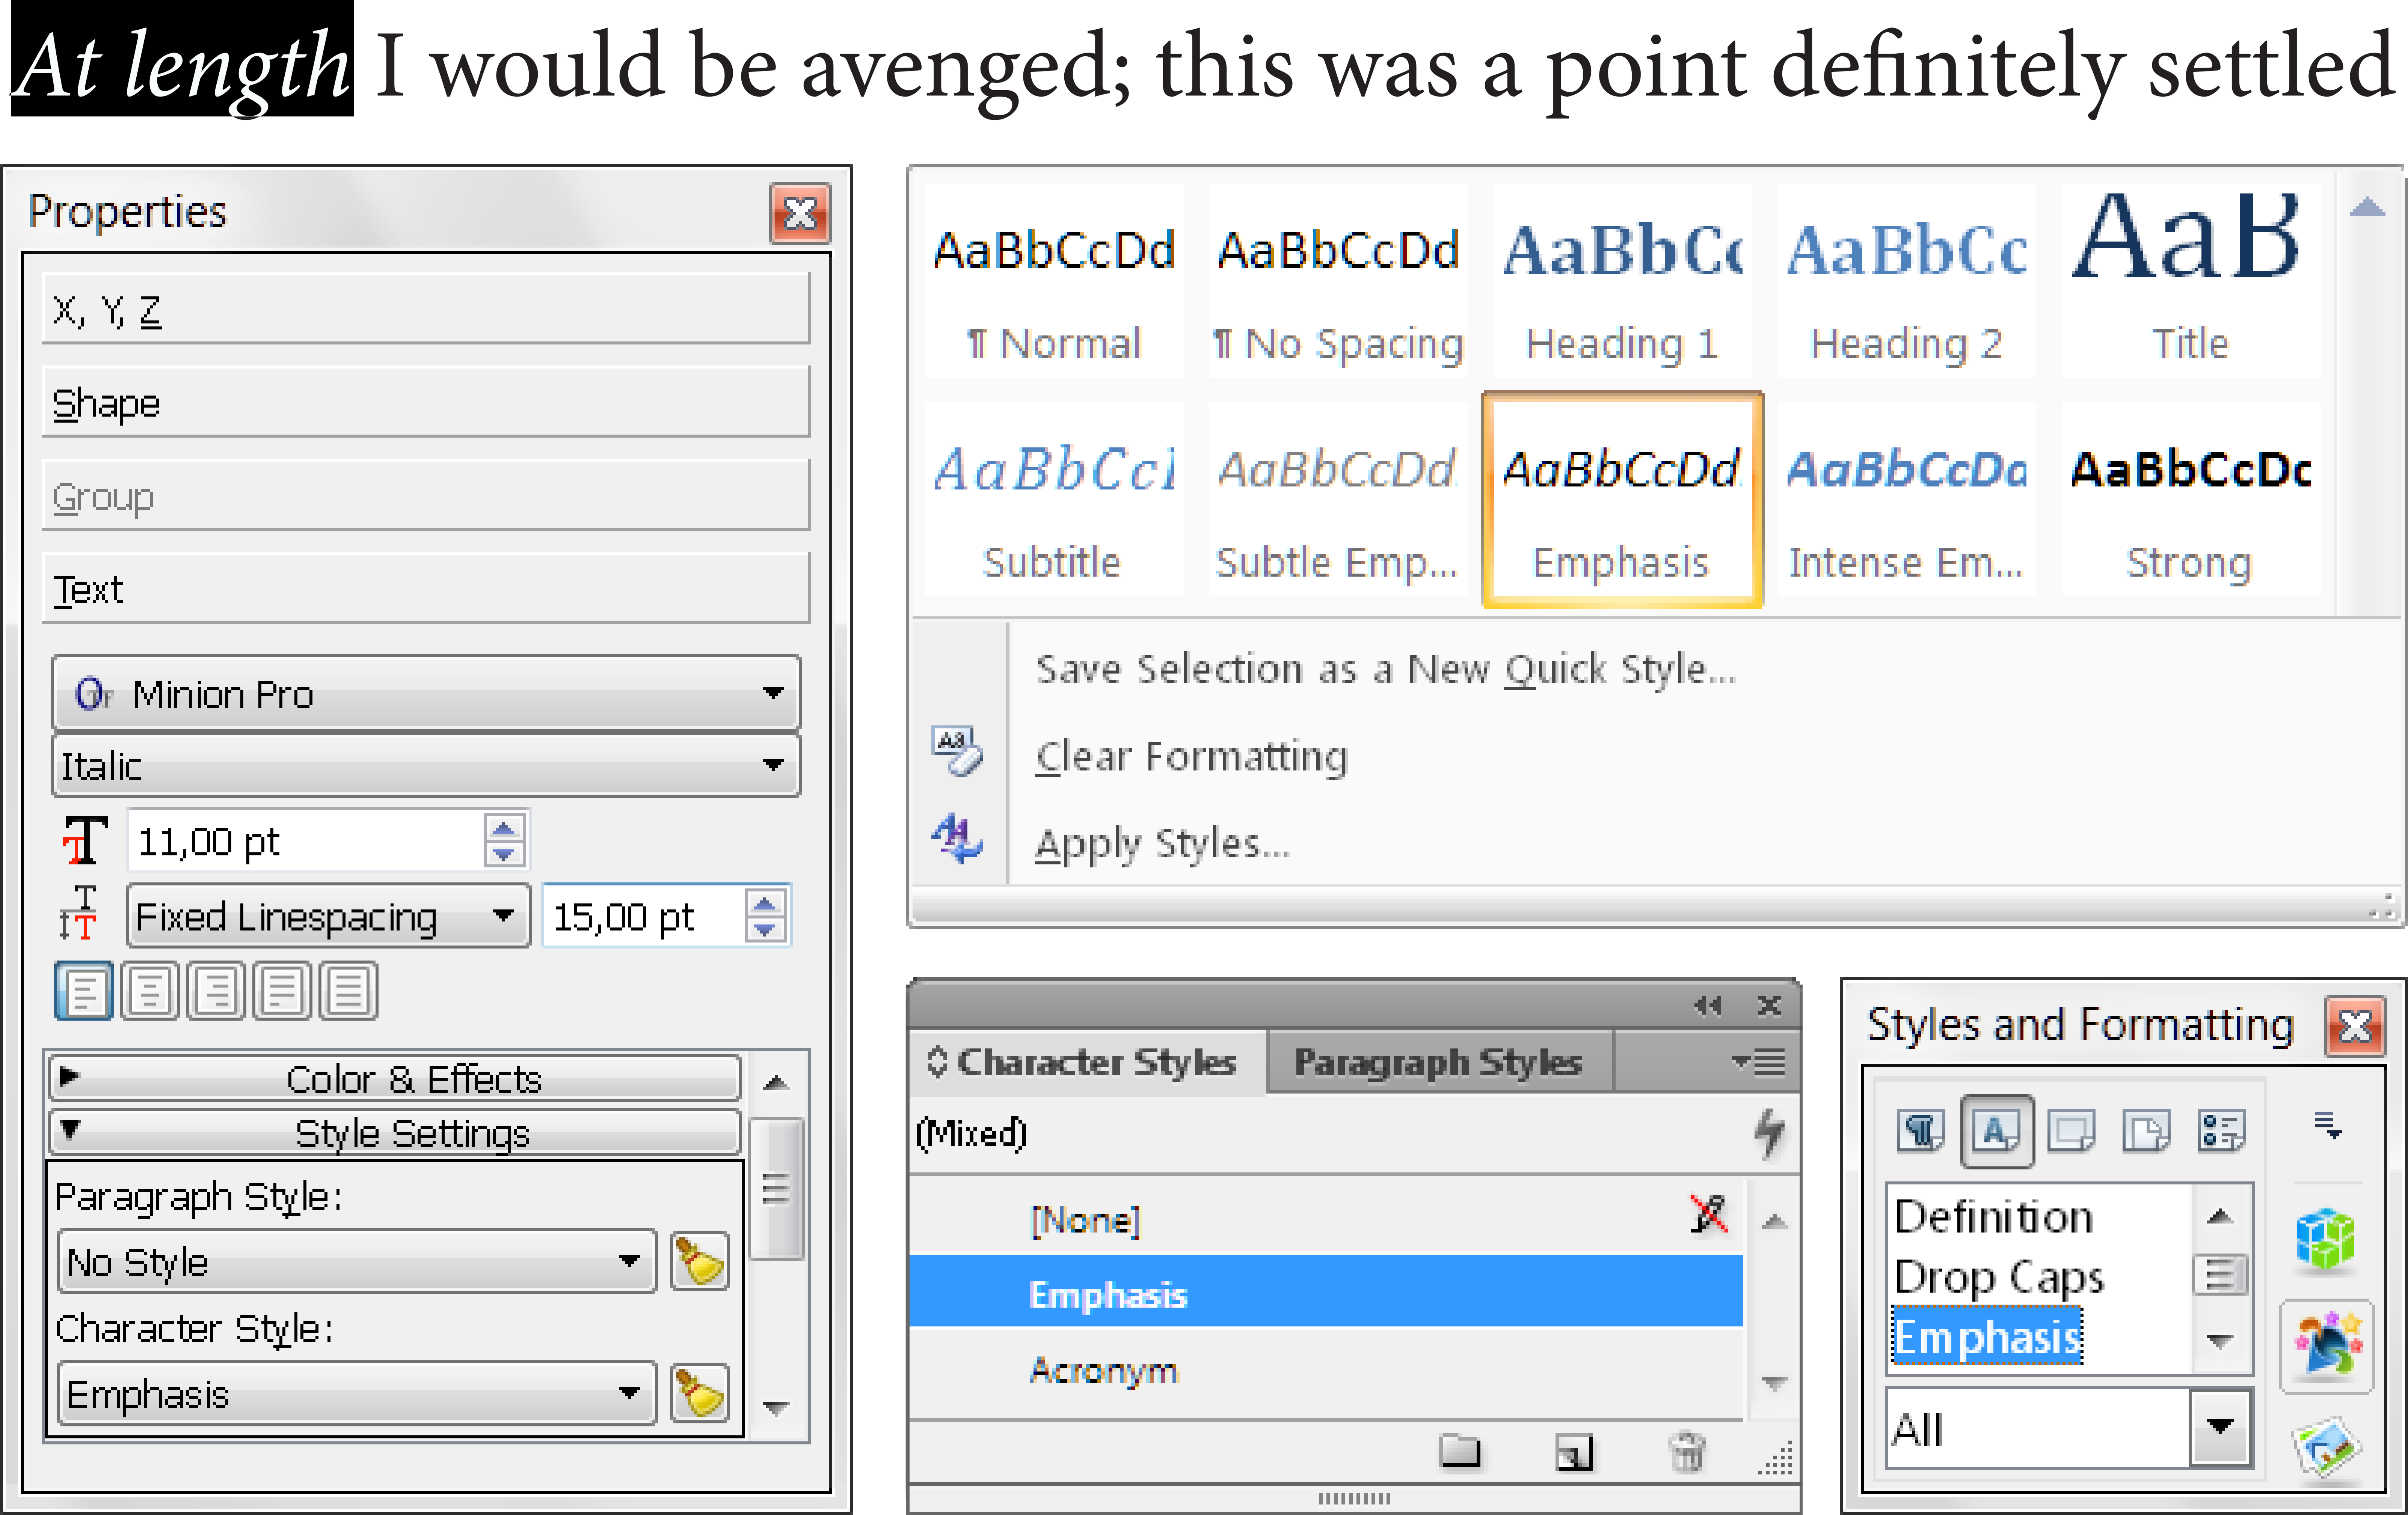
\includegraphics[width=\textwidth]{examples/02/interactive-editors.png}
  \caption{Logical markup in the interactive \acropl{DPS} of \inx{Scribus}
    (left), \inx{Microsoft Word} (above), \inx{Adobe InDesign} (below left) and
    \inx{Apache OpenOffice} (below right)}
\end{figure}

\section{Lightweight Markup Languages}
Parallel to the heavy-duty applications of \acronym{SGML} and \acronym{XML},
there runs a vein of markup languages that give priority to unobtrusiveness and
legibility over expressiveness and genericity. Rooted in the reality of
computer text terminals with limited formatting capabilities, \termpl{lightweight
markup language} leverage punctuation and
indentation to produce comparatively weak and domain-specific, but also humane,
highly intuitive, and often profoundly beautiful markup that is easy to both
read and write. Examples of lightweight markup languages include \inx{Markdown},
\inx{Creole}, \inx{AsciiDoc}, \inx{MakeDoc}, \inx{Setext}, or \inx{Wikicode}.
Lightweight markup languages are typically supplemented by tools that enable
the conversion to more general languages such as \acronym{HTML}. Also typical
is the existence of numerous flavors of every lightweight markup language,
which represent different use cases.

\chapter{Design}
% XML -- CSS, XSL, XSLT
\chapter{Typesetting}
% Accessibility -- WCAG
% Digital Typesetting Pocket Primer, Ron Goldberg
% Word processors do offer typographic primitives
%   <http://word.tips.net/T001081_Inserting_a_Non-Breaking_Space.html>
%   Unicode characters:
%     * \hexa{FEFF} -- \unichar{Zero width no-break space}
%     * \hexa{00A0} -- \unichar{Non-breaking space}
%     * \hexa{200B} -- \unichar{Zero width space}
%     * \hexa{0020} -- \unichar{Space}
%     * \hexa{2009} -- \unichar{Thin space}
%     * ... <http://www.fileformat.info/info/unicode/category/Zs/list.htm>
%     * ... <http://www.fileformat.info/search/google.htm?q=zero+width&domains=www.fileformat.info&sitesearch=www.fileformat.info&client=pub-6975096118196151&forid=1&channel=1657057343&ie=UTF-8&oe=UTF-8&cof=GALT%3A%23008000%3BGL%3A1%3BDIV%3A%23336699%3BVLC%3A663399%3BAH%3Acenter%3BBGC%3AFFFFFF%3BLBGC%3A336699%3BALC%3A0000FF%3BLC%3A0000FF%3BT%3A000000%3BGFNT%3A0000FF%3BGIMP%3A0000FF%3BFORID%3A11&hl=en>
%     * ... <http://www.unicode.org/versions/Unicode1.0.0/V2ch01.pdf>, page 6
%
%%% Hyphenation in HTML
%%%   <http://www.cs.tut.fi/~jkorpela/shy.html>
%%%   <https://developer.mozilla.org/en-US/docs/Web/CSS/hyphens>
\chapter{Release}
\section{Proofreading}
\section{Printing and Binding}
\section{Distribution}
\backmatter

% Bibliography
\printbibliography[heading=bibintoc]

% Acronyms
\fakechapter{Acronyms}
\printacronyms[heading=none]

% Index
\cleardoublepage
\def\index#1{} % Disable indexing
\printindex    % Print the index
\faketoc{Index}

\end{document}
